\documentclass[crop,tikz]{standalone}
\usepackage{pgfplots}

% http://pgfplots.net/tikz/examples/bell-curve/
\pgfplotsset{compat=1.8}
\pgfmathdeclarefunction{gauss}{2}{\pgfmathparse{1/(sqrt(#2*2*pi))*exp(-((x-#1)^2)/(2*#2))}}
\pgfmathdeclarefunction{multigauss}{4}{\pgfmathparse{1/(sqrt(#2*2*pi))*exp(-((x-#1)^2)/(2*#2)) * 1/(sqrt(#4*2*pi))*exp(-((y-#3)^2)/(2*#4))}}

\pgfplotsset{colormap={whiteblack}{color(0cm)=(white); color(1cm)=(gray)}}

\usetikzlibrary{positioning,shapes,arrows}

\begin{document}
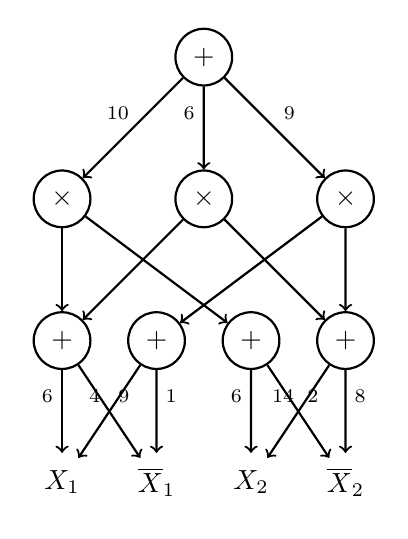
\begin{tikzpicture}
    [scale=.6,auto=left,every node/.style={draw, thick, circle, inner sep = 0pt, minimum width = 0.72cm}]
  \node (n1) at (5,10) {$+$};
  \node (n2) at (2,7) {$\times$};
  \node (n3) at (5,7) {$\times$};
  \node (n4) at (8,7) {$\times$};
  \node (n5) at (2,4) {$+$};
  \node (n6) at (4,4) {$+$};
  \node (n7) at (6,4) {$+$};
  \node (n8) at (8,4) {$+$};
  \node[draw=none] (n9) at (2,1) {$X_1$};
  \node[draw=none] (n10) at (4,1) {$\overline{X}_1$};
  \node[draw=none] (n11) at (6,1) {$X_2$};
  \node[draw=none] (n12) at (8,1) {$\overline{X}_2$};

  \foreach \from/\to/\weight/\pos in {n1/n2/10/above left, n1/n3/6/above left, n1/n4/9/above right, n5/n9/6/above left, n5/n10/4/above left, n6/n9/9/above right, n6/n10/1/above right, n7/n11/6/above left, n7/n12/14/above left, n8/n11/2/above right, n8/n12/8/above right}
    \draw (\from) edge[->, thick] node[\pos, draw=none, circle=none, minimum width=0.5cm, minimum height=0.2cm, inner sep=2pt]{\scriptsize \weight} (\to);

  \foreach \from/\to in {n2/n5, n2/n7, n3/n5, n3/n8, n4/n6, n4/n8}
    \draw (\from) edge[->, thick] (\to);
\end{tikzpicture}
\end{document}
